\documentclass[]{article}
\usepackage{lmodern}
\usepackage{amssymb,amsmath}
\usepackage{ifxetex,ifluatex}
\usepackage{fixltx2e} % provides \textsubscript
\ifnum 0\ifxetex 1\fi\ifluatex 1\fi=0 % if pdftex
  \usepackage[T1]{fontenc}
  \usepackage[utf8]{inputenc}
\else % if luatex or xelatex
  \ifxetex
    \usepackage{mathspec}
  \else
    \usepackage{fontspec}
  \fi
  \defaultfontfeatures{Ligatures=TeX,Scale=MatchLowercase}
\fi
% use upquote if available, for straight quotes in verbatim environments
\IfFileExists{upquote.sty}{\usepackage{upquote}}{}
% use microtype if available
\IfFileExists{microtype.sty}{%
\usepackage{microtype}
\UseMicrotypeSet[protrusion]{basicmath} % disable protrusion for tt fonts
}{}
\usepackage[margin=1in]{geometry}
\usepackage{hyperref}
\hypersetup{unicode=true,
            pdftitle={Data visualization},
            pdfauthor={John M. Drake \& Ana I. Bento},
            pdfborder={0 0 0},
            breaklinks=true}
\urlstyle{same}  % don't use monospace font for urls
\usepackage{color}
\usepackage{fancyvrb}
\newcommand{\VerbBar}{|}
\newcommand{\VERB}{\Verb[commandchars=\\\{\}]}
\DefineVerbatimEnvironment{Highlighting}{Verbatim}{commandchars=\\\{\}}
% Add ',fontsize=\small' for more characters per line
\usepackage{framed}
\definecolor{shadecolor}{RGB}{248,248,248}
\newenvironment{Shaded}{\begin{snugshade}}{\end{snugshade}}
\newcommand{\KeywordTok}[1]{\textcolor[rgb]{0.13,0.29,0.53}{\textbf{#1}}}
\newcommand{\DataTypeTok}[1]{\textcolor[rgb]{0.13,0.29,0.53}{#1}}
\newcommand{\DecValTok}[1]{\textcolor[rgb]{0.00,0.00,0.81}{#1}}
\newcommand{\BaseNTok}[1]{\textcolor[rgb]{0.00,0.00,0.81}{#1}}
\newcommand{\FloatTok}[1]{\textcolor[rgb]{0.00,0.00,0.81}{#1}}
\newcommand{\ConstantTok}[1]{\textcolor[rgb]{0.00,0.00,0.00}{#1}}
\newcommand{\CharTok}[1]{\textcolor[rgb]{0.31,0.60,0.02}{#1}}
\newcommand{\SpecialCharTok}[1]{\textcolor[rgb]{0.00,0.00,0.00}{#1}}
\newcommand{\StringTok}[1]{\textcolor[rgb]{0.31,0.60,0.02}{#1}}
\newcommand{\VerbatimStringTok}[1]{\textcolor[rgb]{0.31,0.60,0.02}{#1}}
\newcommand{\SpecialStringTok}[1]{\textcolor[rgb]{0.31,0.60,0.02}{#1}}
\newcommand{\ImportTok}[1]{#1}
\newcommand{\CommentTok}[1]{\textcolor[rgb]{0.56,0.35,0.01}{\textit{#1}}}
\newcommand{\DocumentationTok}[1]{\textcolor[rgb]{0.56,0.35,0.01}{\textbf{\textit{#1}}}}
\newcommand{\AnnotationTok}[1]{\textcolor[rgb]{0.56,0.35,0.01}{\textbf{\textit{#1}}}}
\newcommand{\CommentVarTok}[1]{\textcolor[rgb]{0.56,0.35,0.01}{\textbf{\textit{#1}}}}
\newcommand{\OtherTok}[1]{\textcolor[rgb]{0.56,0.35,0.01}{#1}}
\newcommand{\FunctionTok}[1]{\textcolor[rgb]{0.00,0.00,0.00}{#1}}
\newcommand{\VariableTok}[1]{\textcolor[rgb]{0.00,0.00,0.00}{#1}}
\newcommand{\ControlFlowTok}[1]{\textcolor[rgb]{0.13,0.29,0.53}{\textbf{#1}}}
\newcommand{\OperatorTok}[1]{\textcolor[rgb]{0.81,0.36,0.00}{\textbf{#1}}}
\newcommand{\BuiltInTok}[1]{#1}
\newcommand{\ExtensionTok}[1]{#1}
\newcommand{\PreprocessorTok}[1]{\textcolor[rgb]{0.56,0.35,0.01}{\textit{#1}}}
\newcommand{\AttributeTok}[1]{\textcolor[rgb]{0.77,0.63,0.00}{#1}}
\newcommand{\RegionMarkerTok}[1]{#1}
\newcommand{\InformationTok}[1]{\textcolor[rgb]{0.56,0.35,0.01}{\textbf{\textit{#1}}}}
\newcommand{\WarningTok}[1]{\textcolor[rgb]{0.56,0.35,0.01}{\textbf{\textit{#1}}}}
\newcommand{\AlertTok}[1]{\textcolor[rgb]{0.94,0.16,0.16}{#1}}
\newcommand{\ErrorTok}[1]{\textcolor[rgb]{0.64,0.00,0.00}{\textbf{#1}}}
\newcommand{\NormalTok}[1]{#1}
\usepackage{graphicx,grffile}
\makeatletter
\def\maxwidth{\ifdim\Gin@nat@width>\linewidth\linewidth\else\Gin@nat@width\fi}
\def\maxheight{\ifdim\Gin@nat@height>\textheight\textheight\else\Gin@nat@height\fi}
\makeatother
% Scale images if necessary, so that they will not overflow the page
% margins by default, and it is still possible to overwrite the defaults
% using explicit options in \includegraphics[width, height, ...]{}
\setkeys{Gin}{width=\maxwidth,height=\maxheight,keepaspectratio}
\IfFileExists{parskip.sty}{%
\usepackage{parskip}
}{% else
\setlength{\parindent}{0pt}
\setlength{\parskip}{6pt plus 2pt minus 1pt}
}
\setlength{\emergencystretch}{3em}  % prevent overfull lines
\providecommand{\tightlist}{%
  \setlength{\itemsep}{0pt}\setlength{\parskip}{0pt}}
\setcounter{secnumdepth}{0}
% Redefines (sub)paragraphs to behave more like sections
\ifx\paragraph\undefined\else
\let\oldparagraph\paragraph
\renewcommand{\paragraph}[1]{\oldparagraph{#1}\mbox{}}
\fi
\ifx\subparagraph\undefined\else
\let\oldsubparagraph\subparagraph
\renewcommand{\subparagraph}[1]{\oldsubparagraph{#1}\mbox{}}
\fi

%%% Use protect on footnotes to avoid problems with footnotes in titles
\let\rmarkdownfootnote\footnote%
\def\footnote{\protect\rmarkdownfootnote}

%%% Change title format to be more compact
\usepackage{titling}

% Create subtitle command for use in maketitle
\newcommand{\subtitle}[1]{
  \posttitle{
    \begin{center}\large#1\end{center}
    }
}

\setlength{\droptitle}{-2em}
  \title{Data visualization}
  \pretitle{\vspace{\droptitle}\centering\huge}
  \posttitle{\par}
  \author{John M. Drake \& Ana I. Bento}
  \preauthor{\centering\large\emph}
  \postauthor{\par}
  \date{}
  \predate{}\postdate{}


\begin{document}
\maketitle

\hypertarget{learning-outcomes}{%
\subsection{Learning outcomes}\label{learning-outcomes}}

\begin{enumerate}
\def\labelenumi{\arabic{enumi}.}
\item
  Add outcome
\item
  Add outcome
\item
  Add outcome
\item
  Add outcome
\end{enumerate}

\hypertarget{introduction}{%
\subsection{Introduction}\label{introduction}}

This is the first in a series of five exercises that constitute
\emph{Training Module 1: Introduction to Scientific Programming}, taught
through the IDEAS PhD program at the University of Georgia Odum School
of Ecology in conjunction with the Center for the Ecology of Infectious
Diseases. This module is based on the premise that computer coding is a
basic scientific skill. This module introduces the principles and
practice of scientific computing with special emphasis on analysis of
infectious disease data. Programming will be done in R. Students will be
taught how to create reproducible research documents using R and R
Markdown and to use git/Github for collaborative and individual
projects. An introduction to scientific programming will teach basic
operations and classes of base R, installation and use of R packages,
data import and transformation, flow control with loops, writing
functions, calculating summary statistics, data visualization, and basic
mapping.

Recommended reading for this module is the book \emph{R for Data
Science} by Hadley Wickham and Garret Grolemund (O'Reilly Media, 2017).

This exercise seeks to introduce the student to basic tasks and
operations required to visualize data in R using \texttt{ggplot2}.
\emph{Data visualization} is a key component of \emph{exploratory data
analysis}. \texttt{ggplot2} implements Leland Wilkinson's idea that
there is a ``grammar of graphics'' -- that is an organizational scheme
based on the semantic replationships among different graphical elements.
Data visualization theory, practice, and exploratory data analysis are
not covered systematically, but rather by example, with the expectation
that students will develop further skills by extending the provided
examples.

\hypertarget{case-study}{%
\subsection{Case study}\label{case-study}}

As a running example in this exercise, we will study a data set on the
spread of Middle East Respiratory Syndrome Corona Virus (MERS-CoV)
compiled and made available by Andrew Rambaut on his Github site
(\url{https://github.com/rambaut/MERS-Cases/blob/gh-pages/data/cases.csv}).
Github is a development platform used by developers to host a wide range
of coding projects and is very popular with data scientists and others
interested in open science. We will return to Github on the final day of
the module. For now, we will just use it to access Rambaut's data.
MERS-CoV is a positive-sense single-stranded Betacoronavirus. Its
closest relatives are the SARS coronavirus, common-cold coronavirus, and
other human betacoronaviruses. MERS-CoV first emerged in Suudi Arabia in
2012. It causes a severe respiratory illness Transmission to humans may
be direct (person-to-person), particularly in hospitals, or from contact
with infected animals. Exposure to camels is associated with many cases,
although bats, particularly the Egyptian Tomb bat (\emph{Taphozous
perforatus}), are suspected to be the maintenance reservoir. The case
fatality rate is around 40\%.

\hypertarget{getting-the-data-into-r}{%
\subsection{Getting the data into R}\label{getting-the-data-into-r}}

To load the MERS data into an R session, do the following:

\begin{enumerate}
\def\labelenumi{\arabic{enumi}.}
\tightlist
\item
  Create a working directory called \texttt{mers}
\item
  Download the file \texttt{cases.csv} and move it to \texttt{mers}
\item
  Open a session of R Studio
\item
  Set the working directory by typing
  \texttt{setwd(\textquotesingle{}\textasciitilde{}/./mers)} where
  \texttt{.} is the file path to your working directory. (Alternatively,
  you can navigate by using the \texttt{Session} drop down menu and
  selecting \texttt{Set\ Working\ Directory}.)
\item
  Create an R \emph{dataframe} by typing
  \texttt{data\ \textless{}-\ read.csv(\textquotesingle{}cases.csv\textquotesingle{})}
  as shown below.
\end{enumerate}

\begin{Shaded}
\begin{Highlighting}[]
\NormalTok{mers <-}\StringTok{ }\KeywordTok{read.csv}\NormalTok{(}\StringTok{'cases.csv'}\NormalTok{)}
\end{Highlighting}
\end{Shaded}

\hypertarget{formatting-some-dates}{%
\subsection{Formatting some dates}\label{formatting-some-dates}}

We can inspect the data using the base R function \texttt{head}. We see
that some variables, such as \texttt{onset} and \texttt{hospitalized}
are dates, but formatted as a \texttt{factor}.

\begin{Shaded}
\begin{Highlighting}[]
\KeywordTok{head}\NormalTok{(mers)}
\end{Highlighting}
\end{Shaded}

\begin{verbatim}
##   number FT KSA_case code gender age country province  city district
## 1      1  2           25M      M  25  Jordan          Zarqa         
## 2      2              30M      M  30  Jordan          Zarqa         
## 3      3  1           40F      F  40  Jordan          Zarqa         
## 4      4              60M      M  60  Jordan          Zarqa         
## 5      5              29M      M  29  Jordan          Zarqa         
## 6      6              33M      M  33  Jordan          Zarqa         
##   prior_travel hospital exposure      onset hospitalized sampled reported
## 1                                2012-03-21   2012-04-04                 
## 2                                2012-03-30   2012-04-08                 
## 3                                2012-04-02   2012-04-09                 
## 4                                2012-04-02                              
## 5                                2012-04-11   2012-04-15                 
## 6                                2012-04-12   2012-04-14                 
##        death discharged comorbidity severity outcome    clinical
## 1 2012-04-25                           fatal   fatal       fatal
## 2                                        CCU            clinical
## 3 2012-04-19                           fatal   fatal       fatal
## 4                                                    subclinical
## 5                                        CCU            clinical
## 6                                        CCU            clinical
##   old_cluster cluster Cauchemez.cluster animal_contact camel_contact   HCW
## 1           A       A                 4          FALSE               FALSE
## 2           A       A                 4          FALSE                TRUE
## 3           A       A                 4          FALSE                TRUE
## 4           A       A                 4          FALSE                TRUE
## 5           A       A                 4                               TRUE
## 6           A       A                 4                               TRUE
##   contact_with            contact secondary suspected inferred    notes
## 1                                                           NA         
## 2            1 health care worker      TRUE      TRUE       NA probable
## 3            1 health care worker      TRUE                 NA         
## 4            1 health care worker      TRUE      TRUE       NA probable
## 5              health care worker      TRUE      TRUE       NA probable
## 6            1 health care worker      TRUE      TRUE       NA probable
##                                                                         citation
## 1 http://applications.emro.who.int/emhj/v19/Supp1/EMHJ_2013_19_Supp1_S12_S18.pdf
## 2 http://applications.emro.who.int/emhj/v19/Supp1/EMHJ_2013_19_Supp1_S12_S18.pdf
## 3 http://applications.emro.who.int/emhj/v19/Supp1/EMHJ_2013_19_Supp1_S12_S18.pdf
## 4 http://applications.emro.who.int/emhj/v19/Supp1/EMHJ_2013_19_Supp1_S12_S18.pdf
## 5 http://applications.emro.who.int/emhj/v19/Supp1/EMHJ_2013_19_Supp1_S12_S18.pdf
## 6 http://applications.emro.who.int/emhj/v19/Supp1/EMHJ_2013_19_Supp1_S12_S18.pdf
##   citation2 citation3 citation4 citation5       sequence accession patient
## 1                                                                        1
## 2                                                                        2
## 3                                         Jordan-N3_2012  KC776174       3
## 4                                                                        4
## 5                                                                        5
## 6                                                                        6
##   speculation  X                                         X.1
## 1             NA http://promedmail.org/direct.php?id=3587349
## 2             NA                                            
## 3             NA                                            
## 4             NA                                            
## 5             NA                                            
## 6             NA
\end{verbatim}

\begin{Shaded}
\begin{Highlighting}[]
\KeywordTok{class}\NormalTok{(mers}\OperatorTok{$}\NormalTok{onset)}
\end{Highlighting}
\end{Shaded}

\begin{verbatim}
## [1] "factor"
\end{verbatim}

These dates can be reformatted using the \texttt{lubridate} package.
Here we create new variables using the \texttt{Date} class. But, first
we correct a few errors.

\begin{Shaded}
\begin{Highlighting}[]
\NormalTok{mers}\OperatorTok{$}\NormalTok{hospitalized[}\DecValTok{890}\NormalTok{] <-}\StringTok{ }\KeywordTok{c}\NormalTok{(}\StringTok{'2015-02-20'}\NormalTok{)}
\NormalTok{mers <-}\StringTok{ }\NormalTok{mers[}\OperatorTok{-}\DecValTok{471}\NormalTok{,]}

\KeywordTok{library}\NormalTok{(lubridate)}
\NormalTok{mers}\OperatorTok{$}\NormalTok{onset2 <-}\StringTok{ }\KeywordTok{ymd}\NormalTok{(mers}\OperatorTok{$}\NormalTok{onset)}
\NormalTok{mers}\OperatorTok{$}\NormalTok{hospitalized2 <-}\StringTok{ }\KeywordTok{ymd}\NormalTok{(mers}\OperatorTok{$}\NormalTok{hospitalized)}
\KeywordTok{class}\NormalTok{(mers}\OperatorTok{$}\NormalTok{onset2)}
\end{Highlighting}
\end{Shaded}

\begin{verbatim}
## [1] "Date"
\end{verbatim}

We may also find it useful to have a simple numerical value for the days
elapsed since the start of the epidemic. We use the following code to
search for the earliest onset date.

\begin{Shaded}
\begin{Highlighting}[]
\NormalTok{day0 <-}\StringTok{ }\KeywordTok{min}\NormalTok{(}\KeywordTok{na.omit}\NormalTok{(mers}\OperatorTok{$}\NormalTok{onset2))}
\end{Highlighting}
\end{Shaded}

\textbf{Question. Why do we use the function \texttt{na.omit}? What
happens if we neglect this command?}

Now we can create a new, numeric value for the ``epidemic day'' for each
case.

\begin{Shaded}
\begin{Highlighting}[]
\NormalTok{mers}\OperatorTok{$}\NormalTok{epi.day <-}\StringTok{ }\KeywordTok{as.numeric}\NormalTok{(mers}\OperatorTok{$}\NormalTok{onset2 }\OperatorTok{-}\StringTok{ }\NormalTok{day0)}
\end{Highlighting}
\end{Shaded}

\textbf{Question. What purpose does the command \texttt{as.numeric}
serve?}

\hypertarget{making-a-plot}{%
\subsection{Making a plot}\label{making-a-plot}}

Next, we load \texttt{ggplot2}.

\begin{Shaded}
\begin{Highlighting}[]
\KeywordTok{library}\NormalTok{(ggplot2)}
\end{Highlighting}
\end{Shaded}

We can explore some of the MERS data using the function \texttt{ggplot}.
One plot we might wish to produce is the \emph{epidemic curve} which is
basically a bar plot. An empty plot can be produced using the command
\texttt{ggplot(data=mers)}. The epidemic curve is then produced by
adding a bar plot using the geom function \texttt{geom\_bar}. The last
line of our code adds some labels.

\begin{Shaded}
\begin{Highlighting}[]
\KeywordTok{ggplot}\NormalTok{(}\DataTypeTok{data=}\NormalTok{mers) }\OperatorTok{+}\StringTok{ }
\StringTok{  }\KeywordTok{geom_bar}\NormalTok{(}\DataTypeTok{mapping=}\KeywordTok{aes}\NormalTok{(}\DataTypeTok{x=}\NormalTok{epi.day)) }\OperatorTok{+}
\StringTok{  }\KeywordTok{labs}\NormalTok{(}\DataTypeTok{x=}\StringTok{'Epidemic day'}\NormalTok{, }\DataTypeTok{y=}\StringTok{'Case count'}\NormalTok{, }\DataTypeTok{title=}\StringTok{'Global count of MERS cases by date of symptom onset'}\NormalTok{,}
       \DataTypeTok{caption=}\StringTok{"Data from: https://github.com/rambaut/MERS-Cases/blob/gh-pages/data/cases.csv"}\NormalTok{)}
\end{Highlighting}
\end{Shaded}

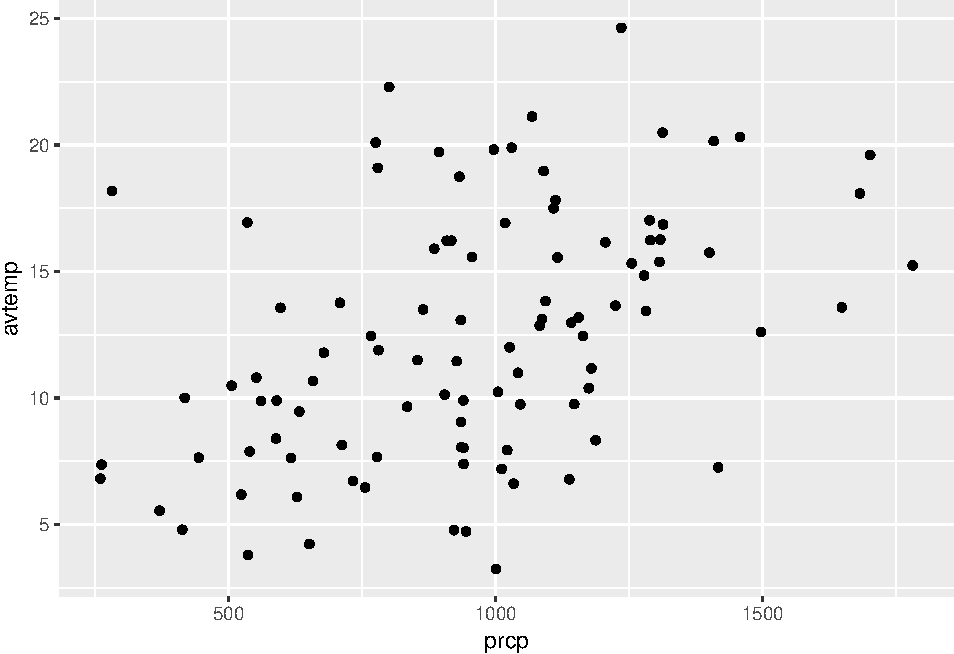
\includegraphics{visualization_files/figure-latex/unnamed-chunk-5-1.pdf}

\textbf{Exercise. To produce this plot, type all the commands up to this
point \emph{exactly} as they appear. Particularly, note that as we
``build'' the plot in the last code snippet, we end each line with the
addition syhmbol ``+''. What happens if we don't use this convention?}

Of course, all these cases are distributed among a number of different
countries. We can modify the plot to show this using the using the
aesthetic \texttt{fill}.

\begin{Shaded}
\begin{Highlighting}[]
\KeywordTok{ggplot}\NormalTok{(}\DataTypeTok{data=}\NormalTok{mers) }\OperatorTok{+}\StringTok{ }
\StringTok{  }\KeywordTok{geom_bar}\NormalTok{(}\DataTypeTok{mapping=}\KeywordTok{aes}\NormalTok{(}\DataTypeTok{x=}\NormalTok{epi.day, }\DataTypeTok{fill=}\NormalTok{country)) }\OperatorTok{+}
\StringTok{  }\KeywordTok{labs}\NormalTok{(}\DataTypeTok{x=}\StringTok{'Epidemic day'}\NormalTok{, }\DataTypeTok{y=}\StringTok{'Case count'}\NormalTok{, }\DataTypeTok{title=}\StringTok{'Global count of MERS cases by date of symptom onset'}\NormalTok{,}
       \DataTypeTok{caption=}\StringTok{"Data from: https://github.com/rambaut/MERS-Cases/blob/gh-pages/data/cases.csv"}\NormalTok{)}
\end{Highlighting}
\end{Shaded}

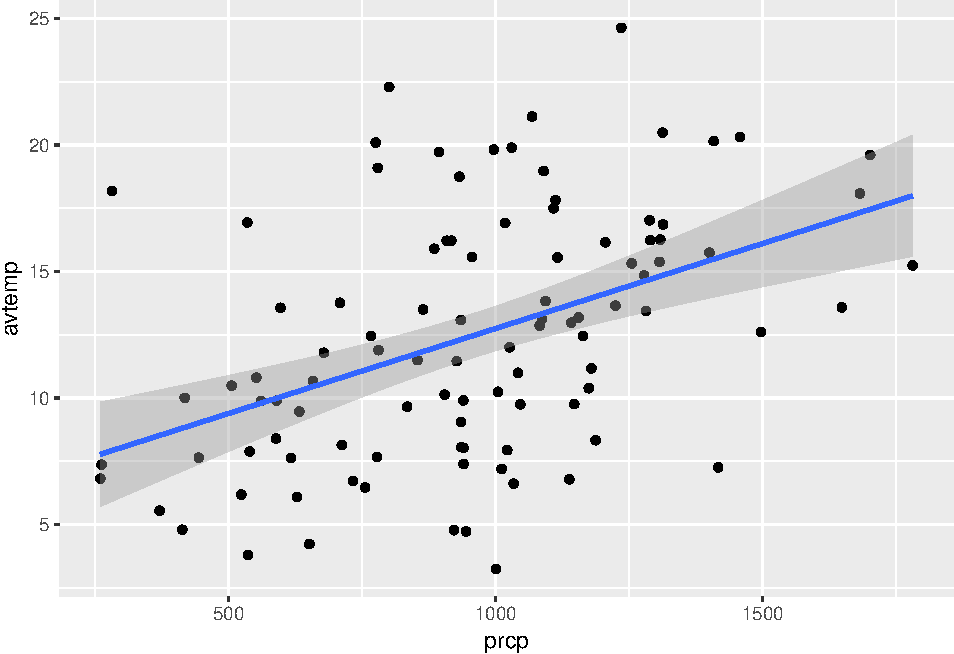
\includegraphics{visualization_files/figure-latex/unnamed-chunk-6-1.pdf}

In this example, we've shown how to make a basic bar plot with
\texttt{ggplot} and the geom function \texttt{geom\_bar}. Our mapping of
data objects to plot objects was performed using \texttt{aes} and we
used the \texttt{fill} aesthetic to examing the distribution of cases
among countries. There are lots of variations on the bar plot that we
can examine. For instance, we can modify the \texttt{position}, which is
another argument to \texttt{geom\_bar}.

\textbf{Exercise. Modify the epidemic curve using the argument
\texttt{position=fill}. What does this plot show?}

\textbf{Exercise. Another way to modify a bar plot is to change the
coordinates. This can be done by ``adding'' \texttt{coord\_flip()} and
\texttt{coord\_polar()} to the plot. Modify the epidemic curve using the
argument \texttt{position=fill}. What does this plot show?}

\hypertarget{univariate-plots}{%
\subsection{Univariate plots}\label{univariate-plots}}

Of course, there are lots of plot types other than bar plots. A quick
reference for some of the more common plot types is the \emph{ggplot2
Cheat Sheet}, available online at
\url{https://www.rstudio.com/wp-content/uploads/2015/03/ggplot2-cheatsheet.pdf}.
To explore some of these plot types, we will first construct a
continuous quantity that is often of interest, the \emph{infectious
period}. From the standpoint of disease transmission, the infectious
period is best defined as the duration of infectiousness for a patient.
From an epidemiological point of view, this may often be approximated as
the time between the onset of symptoms and the time of death,
hospitalization, or isolation. Here we caculate the infectious period
and plot a histogram.

\begin{Shaded}
\begin{Highlighting}[]
\NormalTok{mers}\OperatorTok{$}\NormalTok{infectious.period <-}\StringTok{ }\NormalTok{mers}\OperatorTok{$}\NormalTok{hospitalized2}\OperatorTok{-}\NormalTok{mers}\OperatorTok{$}\NormalTok{onset2    }\CommentTok{# calculate "raw" infectious period}
\KeywordTok{class}\NormalTok{(mers}\OperatorTok{$}\NormalTok{infectious.period)           }\CommentTok{# these data are class "difftime"}
\end{Highlighting}
\end{Shaded}

\begin{verbatim}
## [1] "difftime"
\end{verbatim}

\begin{Shaded}
\begin{Highlighting}[]
\NormalTok{mers}\OperatorTok{$}\NormalTok{infectious.period <-}\StringTok{ }\KeywordTok{as.numeric}\NormalTok{(mers}\OperatorTok{$}\NormalTok{infectious.period, }\DataTypeTok{units =} \StringTok{"days"}\NormalTok{) }\CommentTok{# convert to days}
\KeywordTok{ggplot}\NormalTok{(}\DataTypeTok{data=}\NormalTok{mers) }\OperatorTok{+}
\StringTok{  }\KeywordTok{geom_histogram}\NormalTok{(}\KeywordTok{aes}\NormalTok{(}\DataTypeTok{x=}\NormalTok{infectious.period)) }\OperatorTok{+}\StringTok{ }
\StringTok{  }\KeywordTok{labs}\NormalTok{(}\DataTypeTok{x=}\StringTok{'Infectious period'}\NormalTok{, }\DataTypeTok{y=}\StringTok{'Frequency'}\NormalTok{, }\DataTypeTok{title=}\StringTok{'Distribution of calculated MERS infectious period'}\NormalTok{,}
       \DataTypeTok{caption=}\StringTok{"Data from: https://github.com/rambaut/MERS-Cases/blob/gh-pages/data/cases.csv"}\NormalTok{)}
\end{Highlighting}
\end{Shaded}

\includegraphics{visualization_files/figure-latex/unnamed-chunk-7-1.pdf}

\textbf{Wait a minute! What is a negative infectious period?}

In the case of MERS, this epidemiological definition of infectious
period is misleading, because in some cases the main source of
transmission has been nosocomial (infections in a health care setting).
This appears in our data as a negative time interval between onset and
hospitalization. Perhaps we would wish to calculate a \emph{new} value,
which is the calculated infectious period in the case where it is
positive and zero otherwise. To do this, we rely on the handy function
\texttt{ifelse}.

\begin{Shaded}
\begin{Highlighting}[]
\NormalTok{mers}\OperatorTok{$}\NormalTok{infectious.period2 <-}\StringTok{ }\KeywordTok{ifelse}\NormalTok{(mers}\OperatorTok{$}\NormalTok{infectious.period}\OperatorTok{<}\DecValTok{0}\NormalTok{,}\DecValTok{0}\NormalTok{,mers}\OperatorTok{$}\NormalTok{infectious.period)}
\KeywordTok{ggplot}\NormalTok{(}\DataTypeTok{data=}\NormalTok{mers) }\OperatorTok{+}
\StringTok{  }\KeywordTok{geom_histogram}\NormalTok{(}\KeywordTok{aes}\NormalTok{(}\DataTypeTok{x=}\NormalTok{infectious.period2)) }\OperatorTok{+}\StringTok{ }
\StringTok{  }\KeywordTok{labs}\NormalTok{(}\DataTypeTok{x=}\StringTok{'Infectious period'}\NormalTok{, }\DataTypeTok{y=}\StringTok{'Frequency'}\NormalTok{,}
       \DataTypeTok{title=}\StringTok{'Distribution of calculated MERS infectious period (positive values only)'}\NormalTok{, }\DataTypeTok{caption=}\StringTok{"Data from: https://github.com/rambaut/MERS-Cases/blob/gh-pages/data/cases.csv"}\NormalTok{)}
\end{Highlighting}
\end{Shaded}

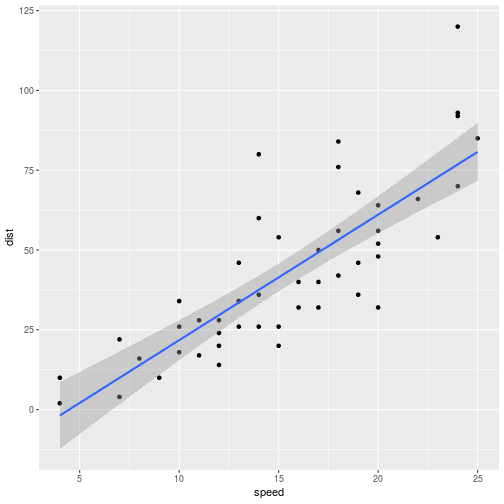
\includegraphics{visualization_files/figure-latex/unnamed-chunk-8-1.pdf}

\textbf{Exercise. Investigate the frequency of hospital-acquired
infections of MERS}

There are lots of different plot types that one can use to inspect
continuously valued or integer-valued data like these. For instance, the
density plot

\begin{Shaded}
\begin{Highlighting}[]
\KeywordTok{ggplot}\NormalTok{(}\DataTypeTok{data=}\NormalTok{mers) }\OperatorTok{+}\StringTok{ }
\StringTok{  }\KeywordTok{geom_density}\NormalTok{(}\DataTypeTok{mapping=}\KeywordTok{aes}\NormalTok{(}\DataTypeTok{x=}\NormalTok{infectious.period2)) }\OperatorTok{+}\StringTok{ }
\StringTok{  }\KeywordTok{labs}\NormalTok{(}\DataTypeTok{x=}\StringTok{'Infectious period'}\NormalTok{, }\DataTypeTok{y=}\StringTok{'Frequency'}\NormalTok{,}
       \DataTypeTok{title=}\StringTok{'Probability density for MERS infectious period (positive values only)'}\NormalTok{, }\DataTypeTok{caption=}\StringTok{"Data from: https://github.com/rambaut/MERS-Cases/blob/gh-pages/data/cases.csv"}\NormalTok{)}
\end{Highlighting}
\end{Shaded}

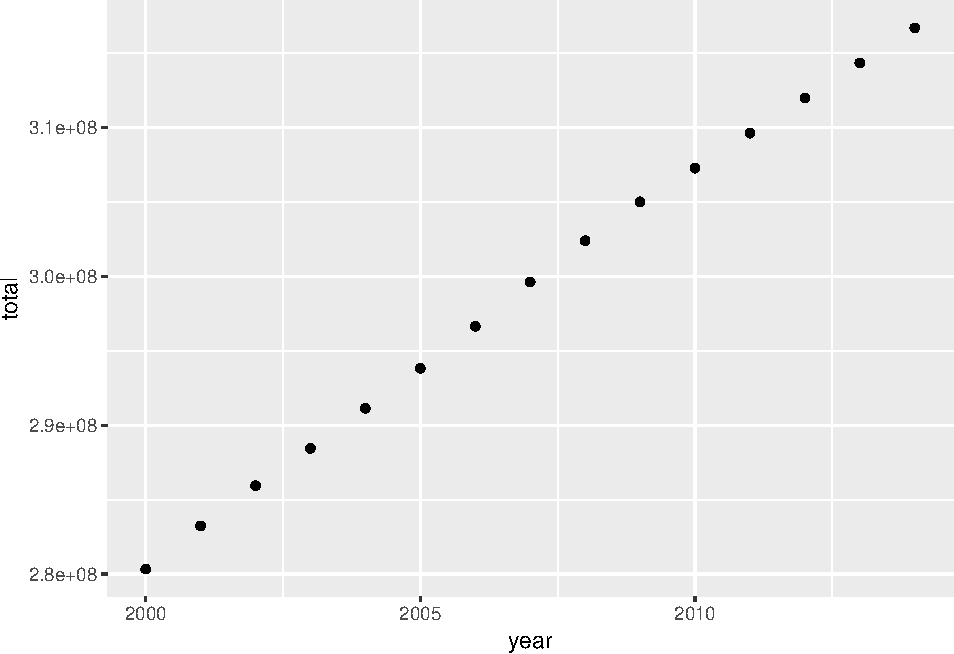
\includegraphics{visualization_files/figure-latex/unnamed-chunk-9-1.pdf}

Or the area plot

\begin{Shaded}
\begin{Highlighting}[]
\KeywordTok{ggplot}\NormalTok{(}\DataTypeTok{data=}\NormalTok{mers) }\OperatorTok{+}\StringTok{ }
\StringTok{  }\KeywordTok{geom_area}\NormalTok{(}\DataTypeTok{stat=}\StringTok{'bin'}\NormalTok{, }\DataTypeTok{mapping=}\KeywordTok{aes}\NormalTok{(}\DataTypeTok{x=}\NormalTok{infectious.period2)) }\OperatorTok{+}
\StringTok{  }\KeywordTok{labs}\NormalTok{(}\DataTypeTok{x=}\StringTok{'Infectious period'}\NormalTok{, }\DataTypeTok{y=}\StringTok{'Frequency'}\NormalTok{,}
       \DataTypeTok{title=}\StringTok{'Area plot for MERS infectious period (positive values only)'}\NormalTok{, }\DataTypeTok{caption=}\StringTok{"Data from: https://github.com/rambaut/MERS-Cases/blob/gh-pages/data/cases.csv"}\NormalTok{)}
\end{Highlighting}
\end{Shaded}

\includegraphics{visualization_files/figure-latex/unnamed-chunk-10-1.pdf}

\textbf{Exercise. Use the infectious period data calculated in
\texttt{mers\$infectious.period2} to experiment with other univariate
plot types like \texttt{geom\_dotplot} and \texttt{geom\_bar}.}

\hypertarget{bivariate-plots}{%
\subsection{Bivariate plots}\label{bivariate-plots}}

The preceding plots have all concerned the distribution of one variable.
Of course, the objective of data analysis is usually to determine the
\emph{relationships} among variables. In this section we study some
plots for two variables.

We can continue our study by focusing on the infectious period.
Epidemiological theory holds that an outbreak will continue to grow in
size as long as the \emph{effective reproduction number} is greater than
one. Roughly, the effective reproduction number is the ration of the
number of transmission events per unit time to the infectious period.
The number of transmission events, in turn, is given by the product of:
(1) the per encounter probability of transmissibility, (2) the contact
rate in the population, and (3) the fraction of the population that is
susceptible to the disease.

This means outbreaks can end two ways. First, the outbreak might ``burn
out'' by infecting such a large fraction of the susceptible population
that the effective reproduction number falls below one. Second,
outbreaks are often curtailed before this point by isolating infected
individuals, effectively by reducing the infectious period. Thus, we
might be interested in understanding how the infectious period changes
over time (i.e., the effectiveness of isolation).

\textbf{Exercise. Use our corrected infectious period variable
(\texttt{infectious.period2}) to study the change in the inectious
period over the course of the MERS epidemic.}

\textbf{Exercise. In data from many outbreaks it can be seen that there
is a kind of \emph{societal learning}. When the infection first emerges
it is not quickly recognized, public health resources have not been
mobilized, it is not known what symptoms are diagnostic, how to treat,
etc. But, quickly, this information is collected and the utbreak is
contained. Is there evidence of this kind of societal learning in the
mers data. Add a curve fit using \texttt{geom\_smooth} to explore this
question. Hint: I solved using the \texttt{loess} method because the
default smoother (gam) failed.}

\textbf{Exercise. Plot \texttt{infectious.period2} against time, as
before, but this time add a separate smooth fit for each country.}

\hypertarget{faceting}{%
\subsection{Faceting}\label{faceting}}

Ordinary plots are great when we want to compare two variables.
Furthermore, we can study three or more variables by varying other
features of the aesthetics (i.e., color). But, as we saw in the last
exercise, when we begin adding information to our plot it can quickly
get cluttered. There are numerous ways to add information from
additional variables, for instance 3-d plots and contour plots. Another
way is to create \emph{multi-panel} plots. In ggplot2, this is called
\emph{faceting}. Faceting allows one to look at subsets of a data set
simultaneously. In ggplot, this is accomplished using the functions
\texttt{facet\_wrap()} and \texttt{facet\_grid}. The behavior of these
functions is shown below. Notice how the second example uses
\texttt{subset} to exclude countries that didn't report many cases and
unusual codings for gender (e.g. \texttt{?M}).

\begin{Shaded}
\begin{Highlighting}[]
\KeywordTok{ggplot}\NormalTok{(}\DataTypeTok{data=}\NormalTok{mers, }\DataTypeTok{mapping=}\KeywordTok{aes}\NormalTok{(}\DataTypeTok{x=}\NormalTok{epi.day, }\DataTypeTok{y=}\NormalTok{infectious.period2)) }\OperatorTok{+}\StringTok{ }
\StringTok{  }\KeywordTok{geom_point}\NormalTok{(}\DataTypeTok{mapping =} \KeywordTok{aes}\NormalTok{(}\DataTypeTok{color=}\NormalTok{country)) }\OperatorTok{+}
\StringTok{  }\KeywordTok{facet_wrap}\NormalTok{(}\OperatorTok{~}\StringTok{ }\NormalTok{country) }\OperatorTok{+}\StringTok{ }
\StringTok{  }\KeywordTok{scale_y_continuous}\NormalTok{(}\DataTypeTok{limits =} \KeywordTok{c}\NormalTok{(}\DecValTok{0}\NormalTok{, }\DecValTok{50}\NormalTok{)) }\OperatorTok{+}
\StringTok{   }\KeywordTok{labs}\NormalTok{(}\DataTypeTok{x=}\StringTok{'Epidemic day'}\NormalTok{, }\DataTypeTok{y=}\StringTok{'Infectious period'}\NormalTok{,}
       \DataTypeTok{title=}\StringTok{'MERS infectious period (positive values only) over time'}\NormalTok{, }\DataTypeTok{caption=}\StringTok{"Data from: https://github.com/rambaut/MERS-Cases/blob/gh-pages/data/cases.csv"}\NormalTok{)}
\end{Highlighting}
\end{Shaded}

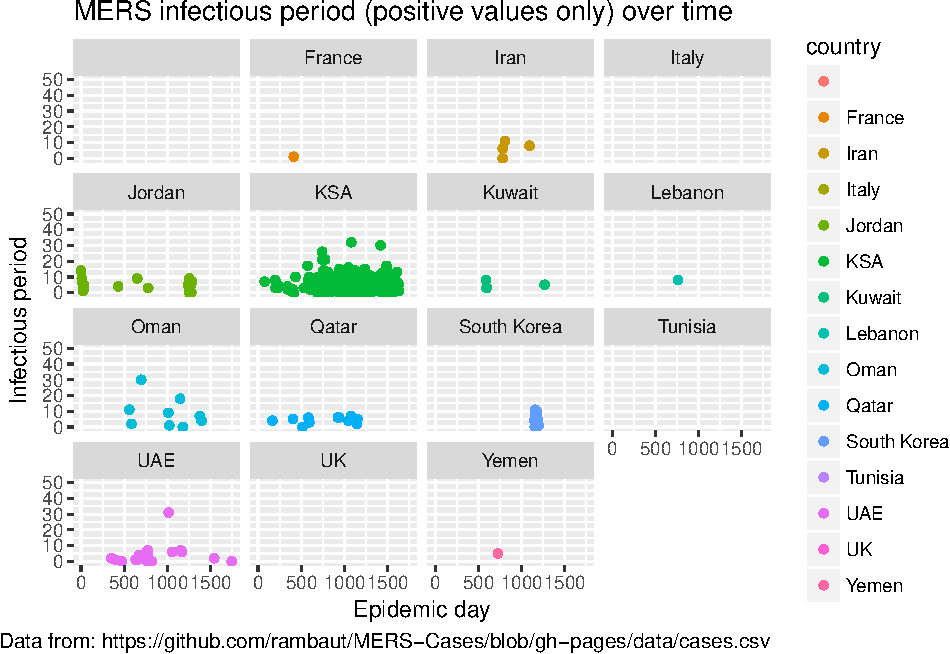
\includegraphics{visualization_files/figure-latex/unnamed-chunk-11-1.pdf}

\begin{Shaded}
\begin{Highlighting}[]
\KeywordTok{ggplot}\NormalTok{(}\DataTypeTok{data=}\KeywordTok{subset}\NormalTok{(mers, gender }\OperatorTok\StringTok{ }\KeywordTok{c}\NormalTok{(}\StringTok{'M'}\NormalTok{, }\StringTok{'F'}\NormalTok{) }\OperatorTok{&}\StringTok{ }\NormalTok{country }\OperatorTok\StringTok{ }\KeywordTok{c}\NormalTok{(}\StringTok{'KSA'}\NormalTok{, }\StringTok{'Oman'}\NormalTok{, }\StringTok{'Iran'}\NormalTok{, }\StringTok{'Jordan'}\NormalTok{, }\StringTok{'Qatar'}\NormalTok{, }\StringTok{'South Korea'}\NormalTok{,}\StringTok{'UAE'}\NormalTok{)), }\DataTypeTok{mapping=}\KeywordTok{aes}\NormalTok{(}\DataTypeTok{x=}\NormalTok{epi.day, }\DataTypeTok{y=}\NormalTok{infectious.period2)) }\OperatorTok{+}\StringTok{ }
\StringTok{  }\KeywordTok{geom_point}\NormalTok{(}\DataTypeTok{mapping =} \KeywordTok{aes}\NormalTok{(}\DataTypeTok{color=}\NormalTok{country)) }\OperatorTok{+}
\StringTok{  }\KeywordTok{facet_grid}\NormalTok{(gender }\OperatorTok{~}\StringTok{ }\NormalTok{country) }\OperatorTok{+}\StringTok{ }
\StringTok{  }\KeywordTok{scale_y_continuous}\NormalTok{(}\DataTypeTok{limits =} \KeywordTok{c}\NormalTok{(}\DecValTok{0}\NormalTok{, }\DecValTok{50}\NormalTok{)) }\OperatorTok{+}
\StringTok{   }\KeywordTok{labs}\NormalTok{(}\DataTypeTok{x=}\StringTok{'Epidemic day'}\NormalTok{, }\DataTypeTok{y=}\StringTok{'Infectious period'}\NormalTok{,}
       \DataTypeTok{title=}\StringTok{'MERS infectious period by gender and country'}\NormalTok{, }\DataTypeTok{caption=}\StringTok{"Data from: https://github.com/rambaut/MERS-Cases/blob/gh-pages/data/cases.csv"}\NormalTok{)}
\end{Highlighting}
\end{Shaded}

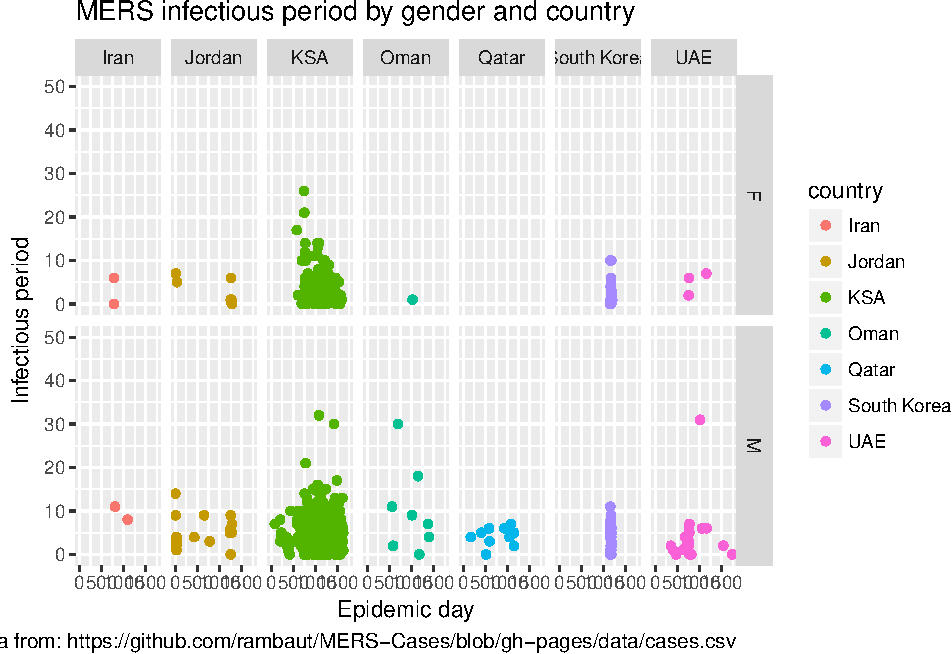
\includegraphics{visualization_files/figure-latex/unnamed-chunk-12-1.pdf}

\textbf{Exercise. Study variation in the \emph{case fatality rate} (the
fraction of cases that end in death) over time and across countries.}

\hypertarget{more}{%
\subsection{More}\label{more}}

The \texttt{ggplot2} package provides over 30 geoms and extension
packages (e.g. \texttt{ggplot2-exts}) provide many others.

\textbf{Exercise. Download and install the ggplot extension. Modify your
plot with one or more new geoms.}

\emph{Interactive graphics} are graphics rendered in HTML that allow the
viewer to extract more information or modify the information presented
using selection, hovering, etc. The \texttt{plotly} package allows the
graphics produced using the vast majority of \texttt{ggplot} functions
to be used interactively using the following sequence:

\begin{enumerate}
\def\labelenumi{\arabic{enumi}.}
\tightlist
\item
  Create a ggplot
\item
  Assign this plot to a variable
\item
  call \texttt{ggplotly} from te \texttt{plotly} package using the
  ggplot as the argument.
\end{enumerate}

The following code demonstrates using the very first graph produced in
this exercise, an epidemic curve created using the barplot geom.

\begin{Shaded}
\begin{Highlighting}[]
\KeywordTok{library}\NormalTok{(plotly)}
\NormalTok{epi.curve <-}\StringTok{ }\KeywordTok{ggplot}\NormalTok{(}\DataTypeTok{data=}\NormalTok{mers) }\OperatorTok{+}\StringTok{ }
\StringTok{  }\KeywordTok{geom_bar}\NormalTok{(}\DataTypeTok{mapping=}\KeywordTok{aes}\NormalTok{(}\DataTypeTok{x=}\NormalTok{epi.day)) }\OperatorTok{+}
\StringTok{  }\KeywordTok{labs}\NormalTok{(}\DataTypeTok{x=}\StringTok{'Epidemic day'}\NormalTok{, }\DataTypeTok{y=}\StringTok{'Case count'}\NormalTok{, }\DataTypeTok{title=}\StringTok{'Global count of MERS cases by date of symptom onset'}\NormalTok{,}
       \DataTypeTok{caption=}\StringTok{"Data from: https://github.com/rambaut/MERS-Cases/blob/gh-pages/data/cases.csv"}\NormalTok{)}
\KeywordTok{ggplotly}\NormalTok{(epi.curve)}
\end{Highlighting}
\end{Shaded}

\textbf{Exercise. Make one of your case fatality plots an interactive
graphic.}


\end{document}
